\documentclass{article}
\usepackage{tikz, comment}
\usepackage{pifont}
\usepackage{fontspec}
\usetikzlibrary{arrows, decorations.markings, decorations.pathreplacing}
\begin{comment}
:Title: Not defined yet
:Tags: pi;;moment;area using polar coordinates, polar integral formula ;cosine, cos ;polar form of a complex number
:Prob: 0.4251;0.421;0.4062;0.4032;0.394
:Author: Prof.Hu Ji-shan, HKUST
:Slug: No name yet

Description Here.........
\end{comment}
\begin{document}\centering

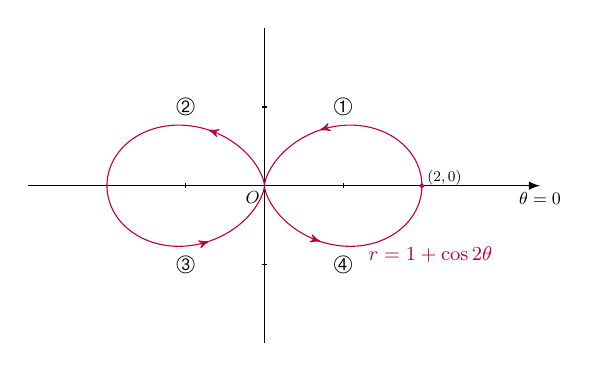
\begin{tikzpicture}[>=latex,xscale=.5*2, yscale=.5*2][font=\sf\small]

%\draw[xstep=1cm,ystep=1cm,color=gray!80] (0, -1) grid (8, 8);

\draw[->] (-3, 0) -- (3.5, 0)node[below, scale=0.7] {$\theta=0$};
\draw[] (0, -2) -- (0,2);

\draw[->, >=stealth', purple, samples=100, smooth, domain=0:1*pi/4, variable=\t]
plot ({(1+cos(2*\t r))*cos(\t r)}, {(1+cos(2*\t r))*sin(\t r)}) -- ({(1+cos(2*(1*pi/4) r))*cos((1*pi/4) r)}, {(1+cos(2*(1*pi/4) r))*sin((1*pi/4) r)});

\foreach \n in {1,3,5}
\draw[->, >=stealth', purple, samples=100, smooth, domain=(\n)*pi/4:(\n+2)*pi/4, variable=\t]
plot ({(1+cos(2*\t r))*cos(\t r)}, {(1+cos(2*\t r))*sin(\t r)}) -- ({(1+cos(2*((\n+2)*pi/4) r))*cos(((\n+2)*pi/4) r)}, {(1+cos(2*((\n+2)*pi/4) r))*sin(((\n+2)*pi/4) r)});

\draw[purple, samples=100, smooth, domain=7*pi/4:2*pi, variable=\t]
plot ({(1+cos(2*\t r))*cos(\t r)}, {(1+cos(2*\t r))*sin(\t r)});


\draw[purple, fill, xscale=1/2, yscale=1/2] ({2*2}, {0*2}) circle(0.05) node[black, right, xshift=0, yshift=3, scale=0.6] {$(2, 0)$};

\node[purple, xshift=60, yshift=-25, scale=0.8] at (0,0) {$r=1+\cos 2\theta$};

\foreach \x in {-1,1}
\draw (\x,2pt/2) -- (\x,-2pt/2)
node[anchor=north] {}%{\tiny$\x$}
;
\foreach \x in {}
\draw (\x,2pt*1.25) -- (\x,-2pt*1.25)
node[anchor=south] {\tiny$\x$}
;
\foreach \y in {-1,1}
\draw (-2pt/2,\y) -- (2pt/2,\y)
node[anchor=east] {}%{\tiny $\y$}
;

\node at ({1}, {1}) {\ding{192}};
\node at ({-1}, {1}) {\ding{193}};
\node at ({-1}, {-1}) {\ding{194}};
\node at ({1}, {-1}) {\ding{195}};

\node[scale=0.7] at (-0.3/2, -0.3/2) {$O$};

\end{tikzpicture}
\end{document}